\documentclass{article}
\usepackage[utf8]{inputenc}
\usepackage{graphicx}

\begin{document}
\title{Day 5}

\author{\emph{Teemu Sarapisto}}
\maketitle

\def\code#1{\texttt{#1}}
\newcommand{\aaa}[3]{%
  \fbox{\includegraphics[height=30mm]{#1}} \quad
  \fbox{\includegraphics[height=30mm]{#2}} \quad
  \fbox{\includegraphics[height=30mm]{#3}} \par}
\newcommand{\bbb}[3]{%
  \medskip\noindent\aaa{#1}{#1-#2}{#1-#3}}

\newpage

\setlength{\fboxsep}{0pt}%

\section{Hands-on}
\begin{figure}[h]
    \centering
    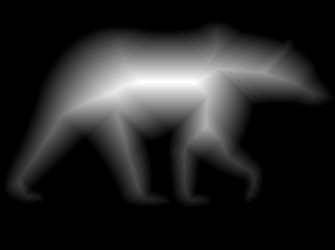
\includegraphics[scale=1.0]{distanced_bear}
\end{figure}

\subsection{Create the object skeleton with OpenCV’s ximgproc.thinning() function from the original image and try if different values for the thinningType argument would make any difference}
Main difference was that some of the thinners didn't create 1px wide lines.

\subsection{Graphing}
\fbox{
\includegraphics[scale=0.60]{bear}} \quad
\fbox{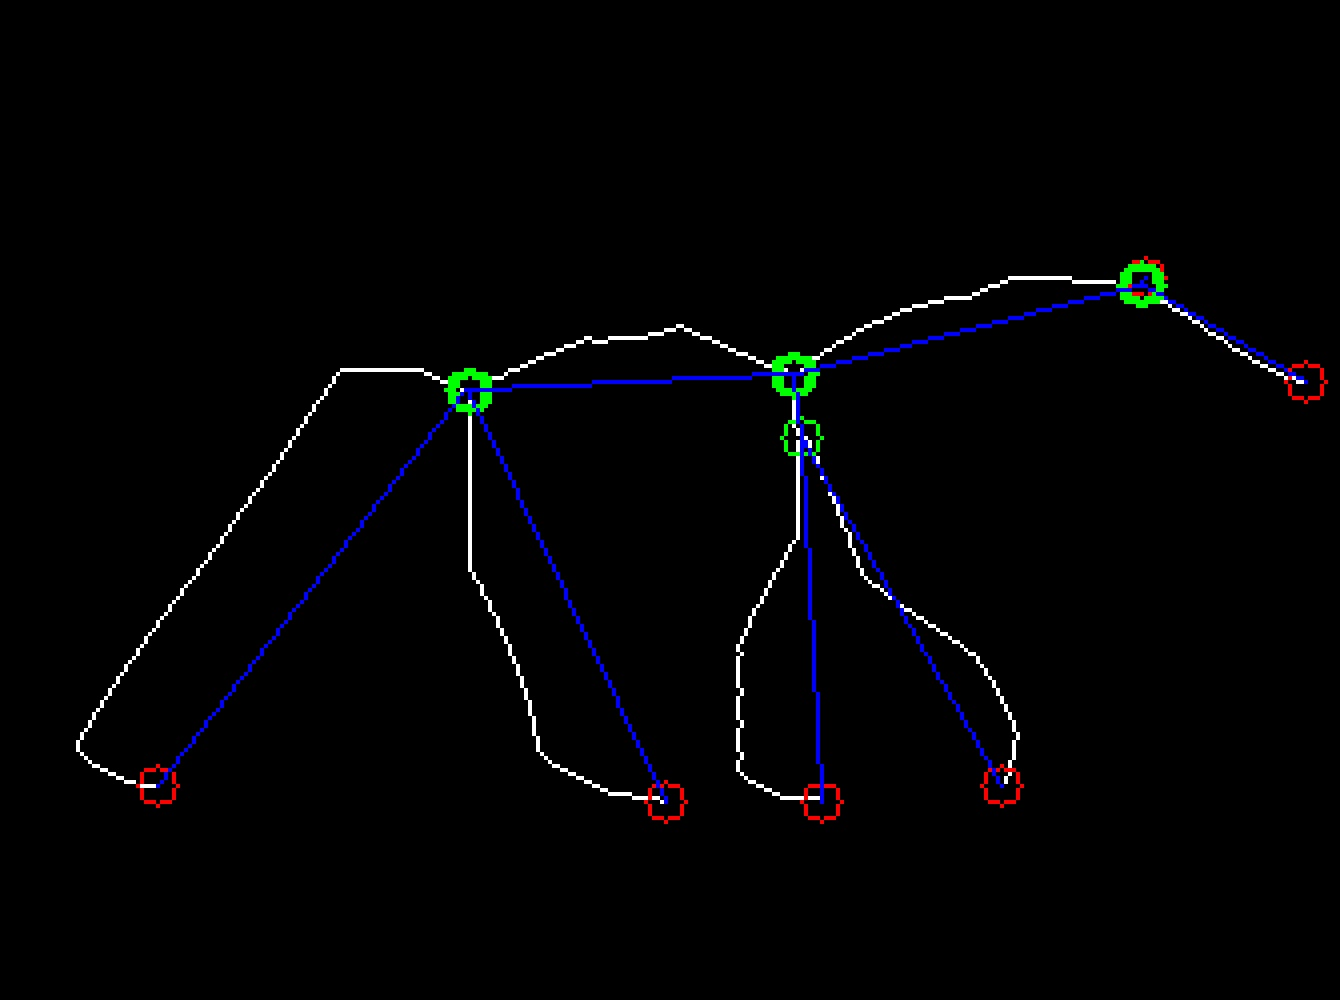
\includegraphics[scale=0.15]{graphed_bear}} \quad

\fbox{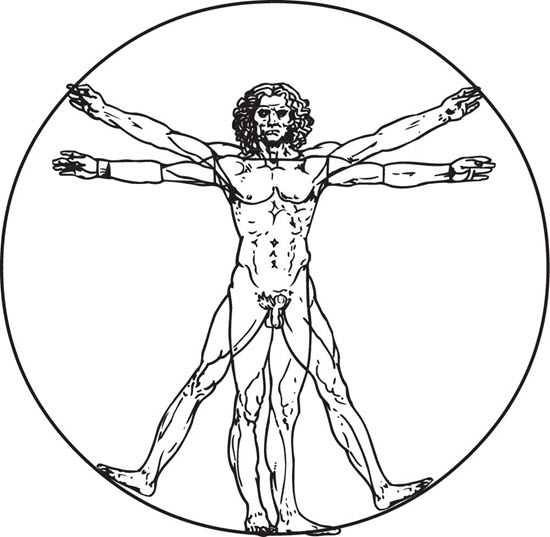
\includegraphics[scale=0.35]{da_vinci_vitruve}} \quad
\fbox{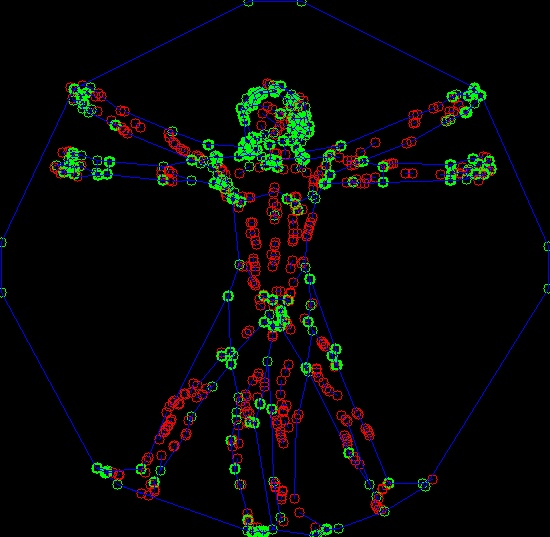
\includegraphics[scale=0.35]{vitruve}} \quad


\fbox{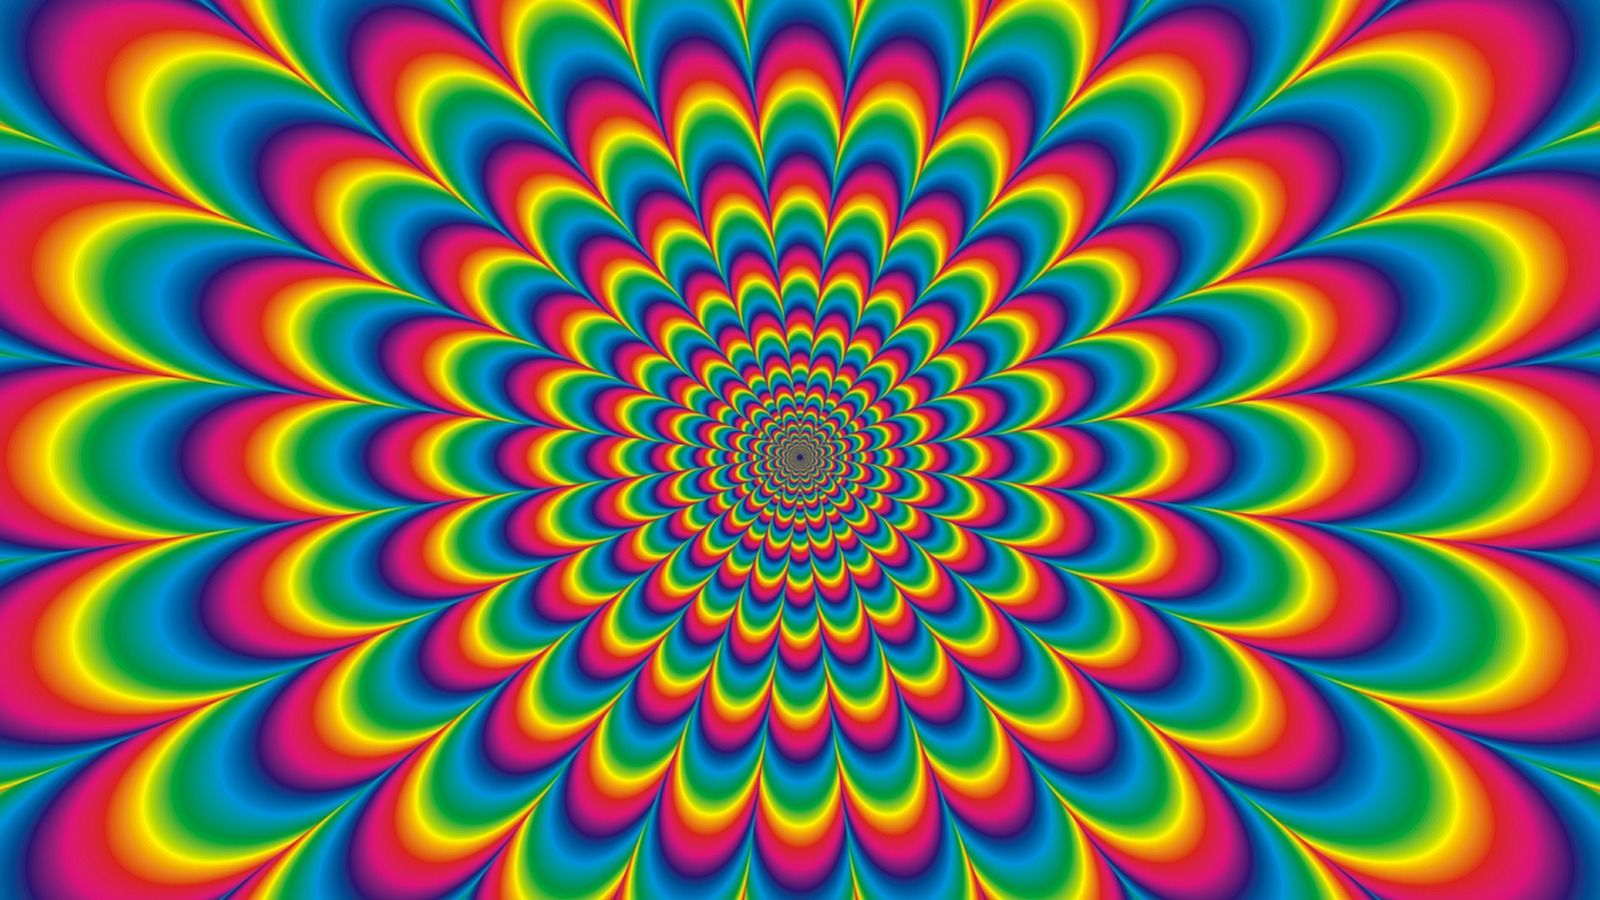
\includegraphics[scale=0.14]{psychedelic_pattern}} \quad
\fbox{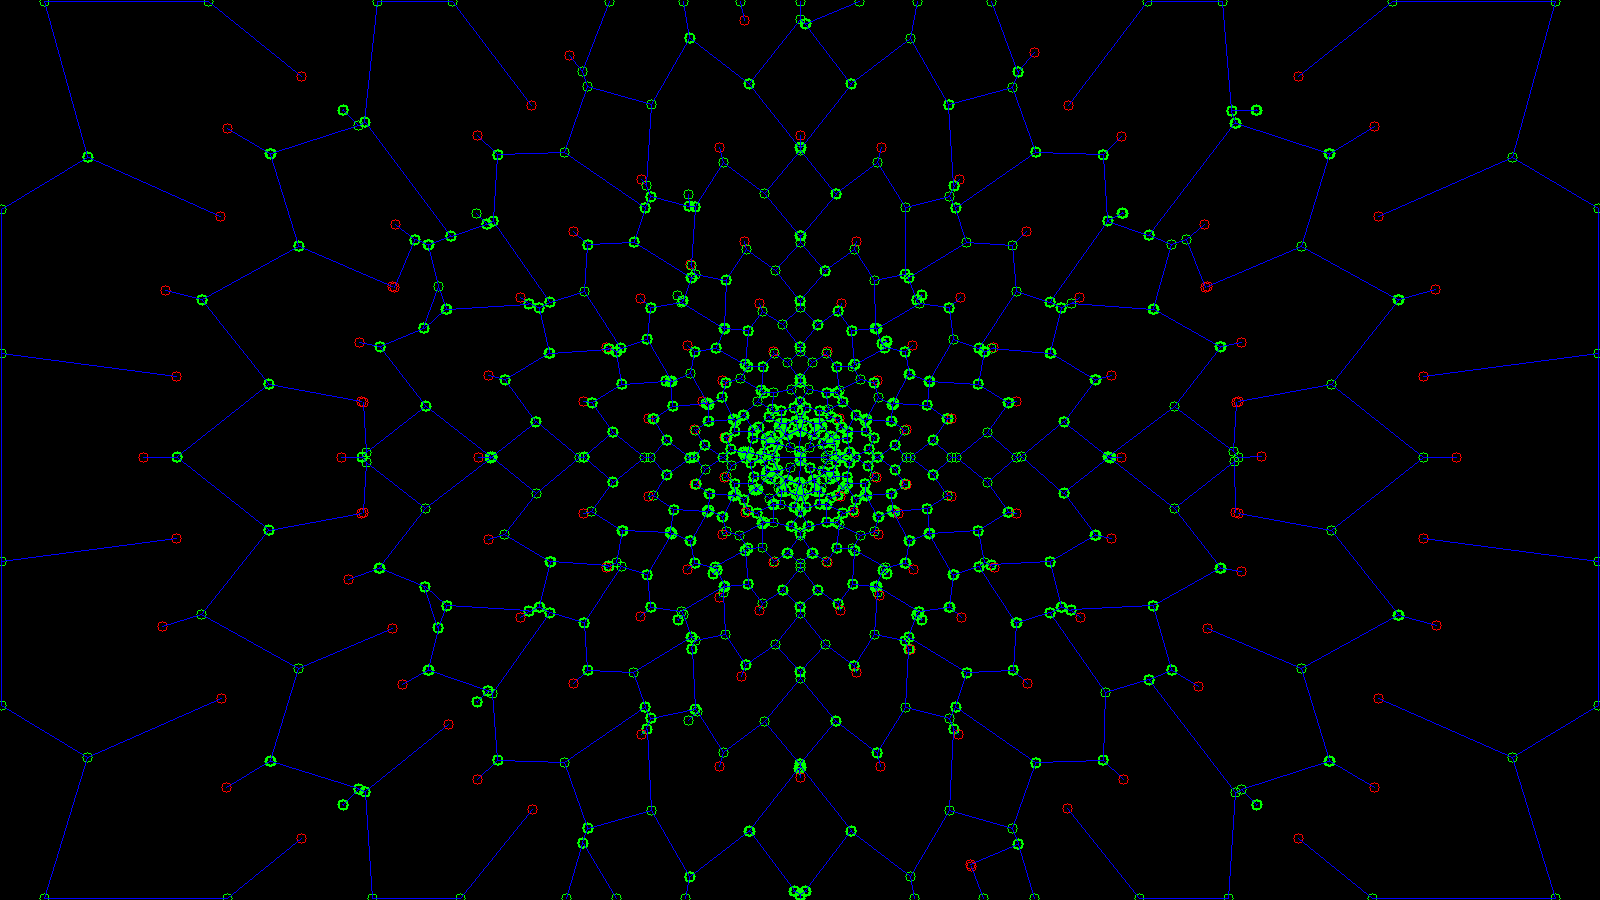
\includegraphics[scale=0.14]{psyke}} \quad

\fbox{
\includegraphics[scale=1.00]{woman_with_umbrella}} \quad
\fbox{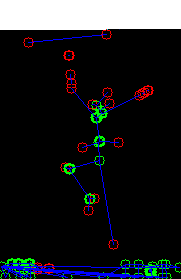
\includegraphics[scale=1.00]{umbrella}} \quad

\fbox{
\includegraphics[scale=0.25]{sacred_derp}} \quad
\fbox{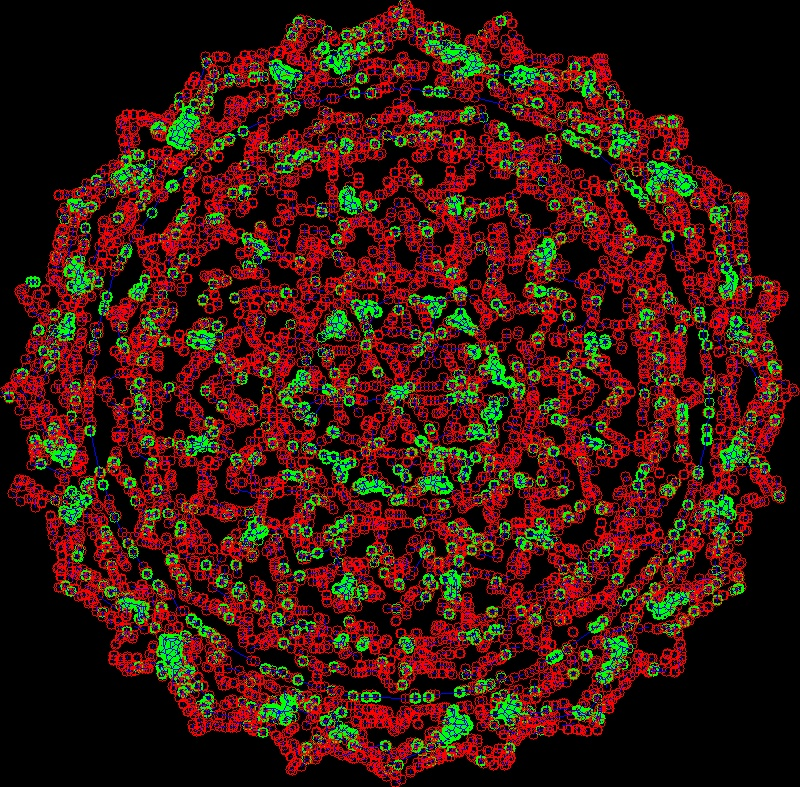
\includegraphics[scale=0.25]{sacred_graph}} \quad

\fbox{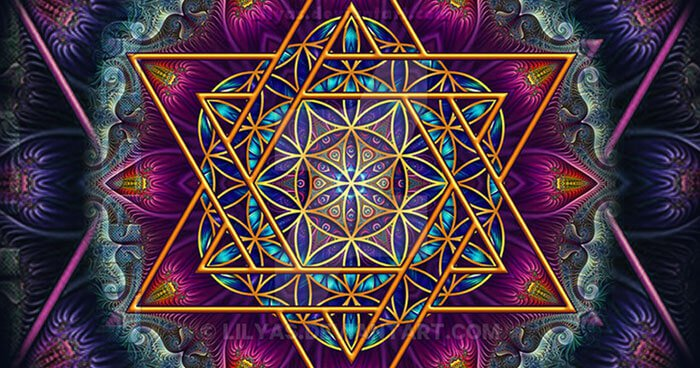
\includegraphics[scale=0.50]{sacred_2}} \quad
\fbox{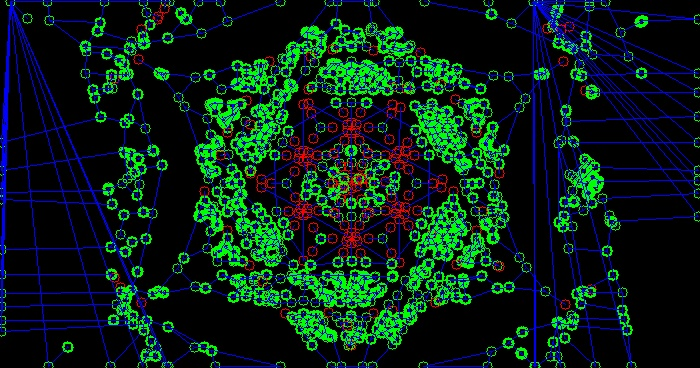
\includegraphics[scale=0.50]{sacred_graph3}} \quad

\subsection{How long it took}
around 4 hours


\section{Homework 3}
42\% classification error with 10k samples.
52.8\% classification error with 1k samples.
\subsection{Code}
\begin{verbatim}
  #! /usr/bin/env python3

  import pickle
  import gzip
  import matplotlib.cm as cm
  import matplotlib.pyplot as plt
  import numpy as np
  import cv2

  with gzip.open('mnist.pkl.gz', 'rb') as fs:
      train_set, valid_set, test_set = pickle.load(fs, encoding='latin1')

  train_x, train_y = train_set
  valid_x, valid_y = valid_set
  test_x,  test_y  = test_set

  def get_pixel_lbp(image, pixel, x, y):
      sum = 0
      if image[x-1, y-1] > pixel: sum += 1
      if image[x-1, y] > pixel: sum += 2
      if image[x-1, y+1] > pixel: sum += 4

      if image[x, y-1] > pixel: sum += 8
      if image[x, y+1] > pixel: sum += 16

      if image[x+1, y-1] > pixel: sum += 32
      if image[x+1, y] > pixel: sum += 64
      if image[x+1, y+1] > pixel: sum += 128
      return sum

  def lbp_histogram(image):
      histogram = np.zeros(256)
      for y, row in enumerate(image):
          if y == 0 or y == image.shape[1] - 1: continue
          for x, cell in enumerate(row):
              if x == 0 or x == image.shape[0] - 1: continue
              histogram[get_pixel_lbp(image, cell, x, y)] += 1
      return histogram

  def train(images):
      results = []
      for image in images:
          hist = lbp_histogram(image.reshape((28, 28)))
          results.append(hist)
      return results

  count = 1000
  results = train(train_x[:count])
  labels = np.asarray(np.arange(0, count), dtype=np.float32).reshape(count, 1)
  for idx, n in enumerate(results):
      labels[idx] = train_y[idx]
  knn = cv2.ml.KNearest_create()

  knn.train(np.asarray(results, dtype=np.float32), cv2.ml.ROW_SAMPLE, labels)

  test_results = train(test_x[:count])
  test_results = np.asarray(test_results, dtype=np.float32)

  ret, predictions, neighbours, dist = knn.findNearest(test_results, k=1)

  success = 0
  for idx, res in enumerate(predictions):
      if int(res[0]) == test_y[idx]:
          success += 1

  print(success / len(predictions))
\end{verbatim}
\subsection{How long it took}
Around 4 hours. Though I was doing something really stupid with creating the labels for the KNN at first, had I not done that I could've easily done it in two hours...
\end{document}
%  LocalWords:  Jorma Laaksonen pdf py tex OpenCV libopencv dev jpg
%  LocalWords:  highgui imgproc imgcodecs greyscale png opencv ing
%  LocalWords:  texlive includegraphics Exactum Gür Ersalan
